%\documentclass[11pt]{scrartcl}
\documentclass[11pt, twoside, a4paper, BCOR8mm, DIV12, bibtotoc,idxtotoc]{scrbook}
\usepackage{german}
\usepackage{typearea}
\usepackage[utf8]{inputenc}
\usepackage{longtable}
\usepackage{hyperref}
\usepackage{graphicx}

% Zusaetzliche Picture-Umgebungen (z.B. shadowenv)
\usepackage{picins}

% Header anpassbar
\usepackage{fancyhdr}

% Headings umdefinieren
\pagestyle{fancy}
\fancyhf{}
\fancyhead[RO]{\nouppercase{\rightmark}}
\fancyhead[LE]{\nouppercase{\leftmark}}
\fancyfoot[RO, LE]{\thepage}

%\addtolength{\headwidth}{\marginparsep}
%\addtolength{\headwidth}{\marginparwidth}
\addtolength{\headwidth}{1cm}

\parindent0.0mm
\parskip0.3cm    
\typearea{13}

\begin{document}

\frontmatter

\begin{titlepage}

\begin{center}
\rule[-.1in]{16cm}{1mm}\\[3mm]
{\fontfamily{cmss}\fontseries{bx}\fontshape{n}\fontsize{20}{20pt}\selectfont
  www.openbib.org $\bullet$ OpenBib Rechercheportal}\\[-2mm]
\rule[-.1in]{16cm}{1mm}

\vspace{5cm}

  \textbf{\fontfamily{cmss}\fontseries{bx}\fontshape{n}\fontsize{30}{30pt}\selectfont OpenBib Recherche-Portal\\[3mm] Technische Dokumentation}

  \vspace{2cm}

  Oliver Flimm \texttt{<flimm@openbib.de>}\\
  Stand: 28.5.2006

  \vspace{8cm}

\rule[-.1in]{16cm}{1mm}\\[3mm]
{\fontfamily{cmss}\fontseries{bx}\fontshape{n}\fontsize{20}{20pt}\selectfont
  www.openbib.org $\bullet$ OpenBib Rechercheportal}\\[-2mm]
\rule[-.1in]{16cm}{1mm}

\end{center}

\end{titlepage}

%\thispagestyle{empty}

%\begin{verbatim}


%Copyright (c) 2004-2006 Oliver Flimm <flimm@openbib.org>

%Es wird die Erlaubnis gegeben dieses Dokument zu kopieren, verteilen 
%und/oder zu veraendern unter den Bedingungen der GNU Free
%Documentation License, Version 1.1 oder einer spaeteren, von der Free 
%Software Foundation veroeffentlichten Version; mit den
%Unveraenderlichen Abschnitten DEREN TITEL AUFGEZAEHLT sind, mit den 
%Vorderseitentexten die AUFGEZAEHLT sind, und mit den Rueckseitentexten
%die AUFGEZAEHLT sind. Eine Kopie dieser Lizenz ist in dem Abschnitt 
%enthalten, der mit "GNU Free Documentation License"
%\end{verbatim}

\tableofcontents

\mainmatter


\chapter{Generelle Features}
Um einen schnellen "Uberblick von den F"ahigkeiten und M"oglichkeiten
des OpenBib Recherche-Portals in der Version 2.0 und h"oher zu
bekommen sowie eine Entscheidungshilfe f"ur einen m"oglichen Einsatz
zu geben, beginnt dieses technische Handbuch mit einer Aufz"ahlung der
generellen Features des Portals.

\section{OpenBib ist OpenSource}
Bei dem OpenBib Recherche-Portal handelt es sich um
OpenSource-Software. Damit ist eine maximale Freiheit bei der
Anpassung an die individuellen Anforderungen gew"ahrleistet.
Dar"uber hinaus ist die Eintrittsschwelle in die "Anderung oder
Erweiterung des Portals durch die Verwendung des DBMS Mysql (Model),
des Template Toolkits (View), der Programmiersprache Perl (Controler)
sowie von GNU gettext (I18N/L10N) "au"serst niedrig. Schlie"slich
fallen selbstverst"andlich keine (Lizenz-)Kosten an.


\section{OpenBib basiert auf Standardkomponenten und bibliothekarischen Standards}
OpenBib verwendet durchg"angig Standardkomponenten. Es sind dies
\begin{description}
\item[Apache Webserver mit mod\_perl] Durch die Verwendung des
  meistgenutzten OpenSource Web\-servers der Welt mit mod\_perl ist OpenBib als
  Webanwendung direkt in den Web\-server integriert. Damit wird eine
  schnellstm"ogliche Reaktionszeit f"ur die Webanwendung erreicht.
\item[MySQL DBMS] MySQL ist eines der meist genutzten OpenSource
  Datenbanksysteme. Durch die Verwendung der in MySQL integrierten
  Volltextsuche ist eine sehr schnelle Indizierung und Recherche m"oglich.
\item[Perl] Die Programmiersprache Perl zeichnet sich durch eine weite
  Verbreitung und eine niedrige Eingangsschwelle aus (Motto: There's
  more than one way to do it).
\item[Perl Template Toolkit] Durch das Perl Template Toolkit wird die
  gesamte Darstellung im Re\-cher\-che-Portal realisiert. Durch seine
  Einfachheit aber auch seiner M"achtigkeit kann durch die Abspaltung
  der Ansichts-Komponente an Webdesigner oder Nicht-Programmierer sehr
  gut eine Arbeitsteilung erreicht werden. Im Vergleich zu XSLT ist
  die Learning Curve des Template Toolkits sehr flach, so da"s
  z.B. eine Auslagerung an einen Bibliothekar problemlos m"oglich ist.
\item[CSS] F"ur die Darstellung werden in den Templates vielf"altige
  CSS-Klassen verwendet, die zentral angepasst werden k"onnen.
\item[GNU gettext] F"ur die Anpassung des Portals an andere Sprachen
  hat sich in vielen Projekten (z.B. bei KDE mit mehr als 40
  Sprachversionen) GNU gettext mit seinen Werkzeugen
  bew"ahrt. W"ahrend andere Systeme z.B. numerische Message-Idendifier
  verwenden und dadurch etwaig verwendete Templates unlesbar machen,
  wird bei GNU gettext die jeweilige Meldung in einer Basissprache
  -- bei OpenBib ist dies Deutsch -- mit einem Methodenaufruf
  gekapselt (inkl. weiterer m"oglicher Parameter), so da"s die
  Templates durchschaubar bleiben.
\item[SOAP] F"ur die Kommunikation mit externen Systemen wird das
  Standard-Protokoll SOAP verwendet.
\item[RSS] "Uber RSS-Feeds k"onnen verschiedene Informationen f"ur das
  Gesamtportal bzw. View-basierte Unter-Portale angeboten werden.
\item[UTF-8] Die Darstellung und interne Verarbeitung der Daten
  geschieht im Encoding UTF-8. Damit sind auch Datenbest"ande, die
  nicht auf ISO-8859-1 basieren, vollst"andig integrierbar.
\item[log4Perl] Durch die Verwendung des Logging-Frameworks log4Perl
  (Perl-Pendant zum bekannten log4j aus der Java-Welt) kann zu
  jeder Zeit an jeder Stelle des Portals ein Debugging erfolgen
  bzw. die genaue Abarbeitung verfolgt werden.
\end{description}

Das Datenmodell und das zugrundeliegende Meta-Datenformat basieren auf
dem bibliothekarischen Standard MAB2. Dar"uber hinaus ist seit der
Ur-Version des Recherche-Portals im Jahr 1997 sehr viel
bibliothekarisches Know-How in die Entwicklung mit eingeflossen.


\section{OpenBib ist "uber verschiedene Views bzw. Sichten
  individualisierbar}
Mit OpenBib k"onnen "uber das Merkmal \textit{View}
bzw. \textit{Sicht} ausgehend von einer zentralen Installation mit
geringstem Aufwand individuell gestaltete andere Portale erstellt
werden. Hierzu wird ein einfacher Mechanismus kaskadierender Templates
und Stylesheets verwendet. Dieser Mechanismus funktioniert sowohl
view- wie auch datenbankabh"angig. 

Wird fuer eine Datenbank oder einen View ein anderer Aufbau eines
Templates gew"unscht, so reicht es, ein entsprechendes
Unterverzeichnis anzulegen, das zugeh"orige Standard-Template in das
Unterverzeichnis zu kopieren und dort zu ver"andern. Damit m"ussen nur
die Templates kopiert werden, die effektiv auch anzupassen sind. Dies
gew"ahrleistet eine sehr gute "Ubersicht der get"atigten "Anderungen
zu verschiedenen Sichten und Datenbanken im Gegensatz zu dem h"aufig
verwendeten Ansatz in anderen Portalen grunds"atzlich alle Templates
zu kopieren.

Neben den Templates werden ebenfalls die Stylesheets "uber diesen
Mechanismus individualisierbar gemacht.

"Uber den Mechanismus kaskadierender Templates hinaus k"onnen
datenbankabh"angige (international- bzw. lokalisierbare)
Bezeichner f"ur einzelne Kategorien definiert werden. Damit lassen
sich einzelne Kategorien unter Beibehaltung ihres Datenbankbezeichners
f"ur spezielle thematische Datenbanken (siehe unten z.B. Digitale
Einbandsammlung) 'umetikettieren' -- und dies mehrsprachig.

Konkrete Beispiele sind
\begin{itemize}
\item Das KUG Recherche-Portal\newline (\texttt{http://kug.ub.uni-koeln.de/})
\item Die Digitale Einbandsammlung der USB K"oln\newline (\texttt{http://einbandsammlung.ub.uni-koeln.de/})
\item Die Virtuelle Bibliothek Elise und Helene Richter\newline (\texttt{http://richterbibliothek.ub.uni-koeln.de/})
\end{description}


\section{OpenBib ist modular aufgebaut}
OpenBib ist in seiner derzeitigen Version sehr modular konzipiert
worden. Dies zeigt sich zu allererst in der Verwendung des
MVC-Design-Patterns (Trennung von Modell, View, Controller) sowie der
Auslagerung aller verwendeten Texte in internationalisierbare bzw.
lokalisierbare GNU gettext Message-Kataloge.

Damit k"onnen -- ganz praktisch gesehen -- entsprechende Arbeiten wie
das visuelle Design des Portals (Templates, Stylesheets) oder die
"Ubersetzung der Texte (GNU gettext) an verschiedene -- nicht im
Programmierumfeld zu suchende -- Mitarbeiter ausgelagert werden.

Dar"uber hinaus k"onnen andere Teile modular ausgewechselt werden --
wenn dies gew"unscht wird. So l"a"st sich u.a. die anf"angliche Suche
"uber einen oder alle Kataloge z.B. von der Realisierung "uber eine
MySQL-Volltext-Datenbank auf andere Volltext-Datenbanken oder gar
Suchmaschinentechnologie "andern. Das neue Verfahren mu"s lediglich
die 'Einspr"unge' in den Bibliographischen Teil der MySQL-Datenbank
liefern. Ganz konkret basierten die ersten Versionen in den Jahren
1997-2000 f"ur die anf"angliche Suche auf der Volltextdatenbank \texttt{freeWAIS-sf}.

\section{OpenBib ist flexibel im internen Katalog- bzw. Metadaten-Format}
Das standardm"a"sig verwendete Katalog- bzw. Meta-Datenformat basiert
auf dem deutschen Bibliotheksstandard MAB2. Dennoch ist die
grunds"atzliche Datenbankstruktur von OpenBib nicht auf MAB2 statisch
festgelegt. Sie ist so universell, da"s sich auch andere Datenformate
wie z.B. das anglo-amerikanische MARC21 anstelle von MAB2 verarbeiten
und in der Datenbank ablegen lassen. Selbstverst"andlich w"urde ein
solcher Wechsel verschiedene "Anderungen -- z.B. in den Templates oder
der Konfiguration -- bedingen, eine Anpassung der Datenbank selbst an
ein Format ist jedoch nicht notwendig.

\section{OpenBib bietet viel Flexibilit"at f"ur den Datenimport }
\subsection{Parametrisierbare Schnittstelle}
OpenBib bietet ausgehend vom auf MAB2 basierten Meta-Datenformat eine
f"ur jede Datenbank individualisierbare und parametrisierbare
Importschnittstelle.

Es kann definiert werden
\begin{itemize}
\item welche Kategorien f"ur die Kurztrefferliste optimierend
  aufbereitet werden sollen,
\item welche Kategorien in den einzelnen Normdatenbereichen f"ur
  \begin{itemize}
  \item eine Volltextsuche nutzbar sein sollen,
  \item eine String- bzw. Wortanfangs-Suche nutzbar sein sollen,
  \item die Anfangsrecherche nutzbar sein sollen sowie
  \item grunds"atzlich ignoriert (blacklisted) werden sollen.
  \end{itemize}
\end{itemize}

Kategorieseitig ist die grunds"atzliche Strategie alles zu
importieren, was nicht geblacklisted ist.

Wie schon bei den Templates und den Stylesheets gibt es auch hier
eine Standardkonfiguration, die f"ur alle Datenbanken gilt, f"ur die
nicht explizit eine eigene Konfiguration erstellt wurde.

\subsection{Plugin-Mechanismus f"ur verschiedene Quell-Datenbanktypen}
Ausgehend von einer Standardkonvertierung (Sisis-Format) k"onnen im
Programm f"ur den automatisierten Import an verschiedenen Stellen des
Import-Ablaufes datenbankspezifische Plugins eingebracht werden, in die
man Spezialanpassungen ausgelagern kann. Grundlegende Phasen, in die
man eingreifen kann sind:
\begin{description}
\item[Einsammeln der Daten] An dieser Stelle k"onnen alternative
  Zugriffsmechanismen -- wie z.B. OAI --
  in externe Plugin-Programme ausgelagert werden.
\item[Vorbereitung der Daten] An dieser Stelle k"onnen alternative
  Vorbereitungsaktionen -- wie z.B. Teilkatalogbildung -- in externe
  Plugin-Programme zwischengeschaltet werden.
\item[Konvertierung der Daten] An dieser Stelle k"onnen alternative
  Konvertierungsroutinen -- z.B. in das MAB2 basierte Meta-Datenformat
  -- zwischengeschaltet werden.
\item[Einladen der Daten] An dieser Stelle k"onnen alternative
  Behandlungen der Daten zwischengeschaltet werden.
\end{description}

\section{OpenBib l"a"st sich "uber WebServices an das Lokalsystem koppeln}
"Uber das Teilprojekt Open Library WebServices (OLWS) von OpenBib
k"onnen verschiedene Informationen aus Lokalsystemen (derzeit nur
Sisis SunRise) in das Recherche-Portal eingebunden werden. Es sind
dies
\begin{itemize}
\item Authentifizierung an OpenBib anhand der Kennung und OPAC-Pin im
  jeweiligen Lokalsystem
\item Anzeige der Nutzerdaten (Name, Anschrift, Sperrung, Sperrgrund usw.)
\item Anzeige des Nutzerkontos mit
  \begin{itemize}
  \item Geb"uhren
  \item vorgemerkten Medien
  \item bestellte Medien
  \item ausgeliehene Medien
  \item "uberzogene Medien
  \end{itemize}
\item Anzeige der Exemplardaten (Signatur, Standort, ausgeliehen
  usw.). "Uber diesen Service wird sekundeaktuell der Ausleihstatus zu
  einem Medium in OpenBib bestimmt.
\item Zugriff auf die Katalogdaten ausgehend von
  Katalogschl"usseln. "Uber diesen Service k"onnen Daten"ubernahmen in
  externe Systeme realisiert werden.
\end{itemize}

Aufgrund der Offenheit der Schnittstelle muss sie nicht auf ein
Lokalsystem beschr"ankt bleiben, sondern kann auf andere ausgedehnt
werden.
\section{OpenBib bietet externe Zugriffsschnittstellen}
F"ur die Recherche von au"sen werden verschiedenen
Zugriffsschnittstellen angeboten. Neben einer HTML-basierten
Zugriffsschnittstelle "uber die die Digitale Bibliothek NRW des hbz
sowie das Hochschulmanagement-System UK-Online der Universit"at zu
K"oln angebunden sind, wird eine SOAP-basierte Schnittstelle f"ur die
WebServices-basierte Anbindung bereitgestellt.

Neben dieser Nutzbarkeit von OpenBib durch andere bestehen weitere
Mechanismen, um eine Integration externer Angebote in OpenBib zu
realisieren. So k"onnen bereits get"atigte Suchanfragen z.B. an
externe Datenbanken und Portale weitergeleitet werden (Digitale
Bibliothek, Fernleihe, Aufsatzbestellung, EZB, DBIS, MedPilot) -- im
Falle der Digitalen Bibliothek NRW sogar unter Mitnahme einer etwaig
in OpenBib erfolgten Authentifizierung.

\section{OpenBib verf"ugt "uber eine intelligente Lastverteilung}
Beim Aufruf des Portals wird der Nutzer an einen der verf"ugbaren
OpenBib Portal-Server weitergeleitet. Ma"sgabe f"ur die Weiterleitung
ist die generelle Ansprechbarkeit (connect) und Auslastung des Servers
(load) sowie seine grundlegende Funktionsf"ahigkeit (MySQL).

Die f"ur die Lastverteilung verwendeten Server k"onnen zentral
konfiguriert werden. Damit kann bei Ausfall oder bei
Wartungsarbeiten der jeweilige Server aus der Verteilung
herausgenommen werden, um in aller Ruhe entsprechende Arbeiten
vorzunehmen.

\section{OpenBib realisiert Content- bzw. Catalogue-Enrichment}
"Uber eine zentrale Anreicherungsdatenbank k"onnen zus"atzliche
Inhalte katalog"ubergreifend in die vorhandenen Katalogdaten
eingeblendet werden. Grundlage ist eine vorhandene ISBN/ISSN. Hiermit
ist z.B. die Ergebnisanreicherung mit Inhaltsverzeichnissen
realisierbar. Die Implementation der Ergebnisanreicherung in OpenBib
ist jedoch so allgemein gehalten, da"s sie sich auch mit anderen
'Zusatz'-Informationen nutzen l"asst. So k"onnen beliebige
Informationen wie Abstracts, Stichwortverzeichnisse u."a. dort zentral
abgelegt werden und sind f"ur alle Kataloge des OpenBib-Portals
nutzbar.

\section{OpenBib bietet Neuzugangslisten als RSS-Feeds}
F"ur jeden Katalog k"onnen Neuzugangslisten bereitgestellt werden.
Hierzu bietet sich die XML-basierte RSS-Technologie an. Im Gegensatz
zu einer gew"ohnlichen Pr"asentaton "uber simple Webseiten bieten
RSS-Feeds den Nutzern durch die geschickte Verwaltung "uber
spezialisierte Programme deutlich mehr Nutzungsm"oglichkeiten. So
k"onnen solche Programme sich um die Sichtung der Daten k"ummern,
schon aufgerufene Titel von den noch nicht aufgerufenen farblich
trennen, Informationen archivieren, Data-Mining in Verbindung mit
spezialisierter Suchtechnologie einsetzen usw.

Grundlage f"ur die in den RSS-Feeds angezeigten Informationen ist das
Neuaufnahmedatum im Katalog. Neben einer allgemeinen Neuzugangsliste
(unter der Rubrik RSS in OpenBib) stehen in den einzelnen Titeln auf
Wunsch Verfasser/Personen-, K"orperschafts/Urheber-, Notations- sowie
Schlagwortspezifische Neuzugangslisten als RSS-Feed zur Verf"ugung.
Erkennbar sind sie durch ein orangenes RSS-Icon. Damit k"onnen sich
Nutzer ausgehend von einem gefundenen Titel z.B. "uber thematisch
verwandte -- z.B. im Fall von Notation oder Schlagwort -- informieren
lassen.

F"ur einzelne Sichten in OpenBib k"onnen einzelne Feeds auf Wunsch
sowohl im Kontext einer automatischen Browsererkennung angeboten
werden, wie sie z.B. der Browser Firefox ab der Version 1.5 besitzt
(dynamisches Lesezeichen), oder in Listenform.

\section{OpenBib bietet ein web-basiertes Administrationsinterface}
Die Einrichtung einzelner Datenbanken, Zusammenfassung von Datenbanken
in Views, die Konfiguration der RSS-Feeds sowie eine Beobachtung
aktiver Sessions (Suchanfragen usw.) kann "uber ein web-basiertes
Administrationsinterface erfolgen. Damit l"a"st sich auch eine gro"se
Anzahl an Katalogen unproblematisch konfigurieren.

\section{OpenBib respektiert die Sicherheit seiner Nutzer}

OpenBib ist auch ohne die Aktivierung der sicherheitskritischen
Browser-Sprache JavaScript vollst"andig nutzbar. Ebenso verwendet es
keine Cookies. Damit wird ein sicherheitsbewu"ster Nutzer nicht dazu
gezwungen, f"ur die Verwendung von OpenBib JavaScript in seinem
Browser zu aktivieren.

Ebenso werden Nutzerdaten bei einer Authentifizierung in OpenBib an
einem Bibliothekssystem nach Ende einer Session selbstverst"andlich
wieder gel"oscht.

\chapter{Praxisbeispiel: OpenBib an der USB K"oln}
Anhand des Einsatzes an der USB K"oln sollen die M"oglichkeiten des
OpenBib Recherche-Portals illustriert werden.

OpenBib wird an der USB K"oln als KUG Recherche-Portal eingesetzt. Im
Projekt 'Kölner UniversitätsGesamtkatalog' (KUG) wird unter Mitwirkung
der Universitäts- u. Stadtbibliothek (USB), der Institute und Seminare
sowie der Zentralbibliothek für Medizin (ZBMED) seit Anfang 2002 ein
universitätsweiter bibliothekarischer Gesamtkatalog aufgebaut.

\section{Kataloge und Zahlen}
Mit Ende des Jahres 2005 sind im KUG-Projekt insgesamt 145 Institute
und Seminare neben den Katalogen der USB Köln und der ZBMED
zusammengefasst, von denen wiederum 139 (in 104 Datenbanken) im KUG
Recherche-Portal sichtbar sind. 

Neben den Katalogen der Instituts- und Seminarbibliotheken wurden im
KUG Recherche-Portal weitere Spezialkataloge
erschlossen bzw. erst verwirklicht. Dazu geh"oren die Digitale
Einbandsammlung der USB K"oln, die Virtuelle Bibliothek Elise und
Helene Richter, der Hochschulschriftenserver, EconBiz, das Graph
Drawing Eprint-Archive, die Poetica-Sammlung, die Sammlung K"olner
Zeitungsausschnitte, der Katalog der  Bibliothek des Oratoriums
Kevelaerinense sowie diverse separate Teilkataloge des USB-Bestandes
(Lehrbuchsammlung, Lesesaal, Europ"aisches Dokumentationszentrum).

Insgesamt sind damit im KUG Recherche-Portal 119 verschiedene
Katalogdatenbanken mit derzeit insgesamt 4942543 Titelaufnahmen
vertreten.

\section{Technik}
Das KUG Recherche-Portal wird mit drei Doppel-Pentium-III Servern
(1.16 GHZ CPU, 4 GB RAM) im RAID-Level 1 betrieben. Alle Rechner
werden im Rahmen der Lastverteilung genutzt, wobei einer der drei
Rechner zus"atzlich die eigentliche Verteilung "ubernimmt.

Neben diesen drei Produktions-Servern verf"ugen wir "uber ein Test-
und Entwicklungssytem (300 EUR Standard-Desktop), auf dem vor einem
Upgrade unter Beteiligung unserer Kollegen aus dem Haus bzw. aus den
dezentralen Bibliotheken eine intensive Testphase durchgef"uhrt wird.
Erst wenn keine gravierenden Fehler gemeldet werden erfolgt die
Umstellung der Produktionssysteme.

\section{Betrieb}
\subsection{N"achtlicher Aufbau der Datenbanken}
Alle im Recherche-Portal vorhandenen Daten werden ausgehend von den
jeweiligen Quell-Sys\-te\-men, auf denen die Katalogisierung stattfindet,
n"achtlich aktualisiert. Dazu werden die Daten auf den Quell-Systemen
entladen sowie auf einem gesch"utzten Bereich eines Webservers
abgelegt. Von dort sammeln die einzelnen Server des Recherche-Portals
die Daten automatisiert ein, wandeln sie um und spielen Sie in ihre
lokalen MySQL-Recherchedatenbanken ein.

Unsere Erfahrung mit einem alternativen Recherche-Portal hatte
zwischenzeitlich gezeigt, dass Recherchen direkt auf den
Quell-Systemen die entsprechenden Systeme massiv belasteten -- in den
Modulen Katalogisierung, Erwerbung sowie Ausleihe waren ganz
erhebliche Performance-Probleme zu verzeichnen. Die Entkopplung von
Katalogisierungs- und Recherche-Datenbanken hat sich hier f"ur beide
Seiten als sehr vorteilhaft erwiesen.


\subsection{Datenquellen und -formate}
Neben den Daten der USB, ZBMED sowie der dezentralen Bibliotheken, die
einheitlich aus Sisis SunRise-Systemen stammen, verarbeiten wir f"ur
unsere Spezialkataloge auch andere Daten. So speisen sich die Kataloge unseres
Hochschulschriftenservers (KUPS) sowie des am Lehrstuhl f"ur Informatik
angesiedelten Graph Drawing E-print Archive (GDEA) "uber das
OAI-Syn\-chro\-ni\-sa\-tions\-pro\-to\-koll.

Zus"atzlich k"onnen wir derzeit automatisiert Quelldaten von Lars,
Allegro, Bislok, LIDOS und FileMaker verarbeiten, dazu kommen
abgeleitete Datenformate, die z.T. auf einem einfachen Lars-Derivat
(Kategoriename/Kategorieinhalt) beruhen.

Produktiv setzen wir derzeit jedoch nur ein Lars-Derivat f"ur die
Einbindung des Kataloges des Italienischen Kulturinstituts sowie
unserer Zeitungsausschnitts-Sammlung ein.

%LIDOS und FileMaker sind f"ur UTF-8 Datenbest"ande des Ostasiatischen
%Seminars angedacht, da diese Institute derzeit aufgrund fehlender
%UTF-8 Unterst"utzung nicht in unserem Lokalystem katalogisieren
%k"onnen.

Ausgehend von den USB-Katalogdaten bilden wir verschiedene
abgeschlossene Teilkataloge. Diese basieren entweder auf einem
speziellen Standort (Lehrbuchsammlung, Lesesaal) oder einem speziellen
Ausleih-Nutzer (EDZ, realisiert "uber einen entsprechenden OLWS-Dienst
f"ur das Lokalsystem). Zus"atzlich werden im Falle des EDZ-Katalogs
dessen Daten mit einer speziellen Sachgruppenkategorie angereichert.

Schlie"slich verwenden wir f"ur die Internetquellen der Virtuellen
Fachbibliothek Wirtschaftswissenschaften (EconBiz) eine
SQL-Schnittstelle f"ur den Datenabzug.

Durch die Verwendung eines einheitlichen Meta-Datenformats als
Grundlage k"onnen neue Datenbest"ande sehr einfach in das Portal
integriert werden.


\subsection{Flexibler Einsatz in Projekten}

Durch die vielen M"oglichkeiten der Anpassung war die Software des
Recherche-Portals predestiniert f"ur den Einsatz in weiteren
Projekten\cite{FlimmHoffJB:06}.

Hier sind insbesondere zwei Kataloge zu nennen: Die digitale
Einbandsammlung der USB K"oln sowie die Virtuelle Bibliothek Elise und
Helene Richter.


\subsubsection{Digitale Einbandsammlung der USB K"oln}

Im Projekt 'Digitale Einbandsammlung' wurde an der USB eine
Einbanddatenbank, bestehend aus Einbandbeschreibungen und Bildern der
jeweiligen Einbände, konzipiert und realisiert. Dazu wurde ein
Scan-Workflow erarbeitet und programmtechnisch in einer
eigenentwickelten Kompontente OpenDIA -- die ein weiteres Teilprojekt
von OpenBib ist -- umgesetzt, mit dem die eingescannten Einbandbilder
erfasst, mit Meta-Daten angereichtert und präsentiert werden.

Ausgehend vom KUG Recherche-Portal (OpenBib) wurden diese Abbildungen
samt Daten bei Wahrung der Eigenständigkeit beider Komponten --
OpenBib und OpenDIA -- visuell zu einem Ganzen zusammen gefügt. Diese
visuelle Integration wurde durch die Flexibilit"at beider Komponenten
erst erm"oglicht -- speziell durch die individualisierbaren
Portal-Sichten in OpenBib. 

Durch den pragmatischen Einsatz weitgehend bereits vorhandener,
bekannter sowie beherrschbarer Techniken und Programme bei diesem
Projekt konnte die USB innerhalb von nur 3 Monaten mit einem neuen
interessanten Dienst an die Öffentlichkeit treten. Die feierliche
Präsentation der 'Digitalen Einbandsammlung' geschah dabei im Rahmen
der 10.  Jahrestagung des Arbeitskreises für die Erfassung,
Erschließung und Erhaltung historischer Bucheinbände, die an der USB
Köln vom 22.-24.  September 2005 stattgefunden hat.  Eine
ausf"uhrliche Zusammenfassung der Konzeption und der technischen
Realisierung findet sich in \cite{BoeFli:EinbandDB}.


\subsubsection{Virtuelle Bibliothek Elise und Helene Richter}

Im Projekt 'Virtuelle Bibliothek Elise und Helene Richter', das Teil
der NS-Provenienzforschung in der USB Köln ist, wurde f"ur die
in die von der USB aufgesp"urten Medien aus der ehemaligen Bibliothek
der Schwestern Richter ein eigenst"andiges Recherche-Portal auf Basis
individualisierbarer Portal-Sichten erstellt.

\section{Fazit}

Die Einsatz der eigenentwickelten Portal-Software OpenBib, die
vollständig aus OpenSource-Komponenten aufgebaut ist, hat sich in der
praktischen Arbeit als sehr vorteilhaft erwiesen:

\begin{itemize}
\item Erweiterungen werden umgehend selbständig vorgenommen sowie
  Probleme schneller gelöst.
\item Von unseren Benutzern an uns herangetragene Wünsche werden
  schneller umgesetzt.
\item Release-Zyklen der Software werden selbst vorgegeben.
\item Die Integration mit anderen Software-Produkten über
  standardisierte Schnittstellen ist nun mit wenig Aufwand möglich.
\end{itemize}
    
\chapter{Grundlegende Architektur}

Die OpenBib-Portalsoftware-Suite ist in logischen Schichten
organisiert. Ein Schaubild der ge\-ne\-rellen Architektur zeigt Abb.
\ref{bild:architektur}. Dieses Kapitel soll einen kurzen Abri"s dieser
Architektur geben, damit die gr"o"seren Zusammenh"ange deutlich
werden. Die Schichten von 'unten' nach 'oben' sind: Die
datenbankabh"angige Schicht, die datenbank"ubergreifende Schicht, die
Portal-Schicht mit weiteren externen Zugriffsmechanismen (DigiBib,
UK-Online) und schlie"slich die Lastverteilungs-Schicht. Diese
Schichten werden bei der Interaktion mit einem Benutzer bei der
Verwendung des OpenBib-Portals in entgegengesetzter Richtung von
'oben' nach 'unten' durchlaufen.


\begin{figure}
\begin{shadowenv}
  \vspace{4mm}
    \centering \begin{minipage}[b]{1.0\textwidth}
      \centering 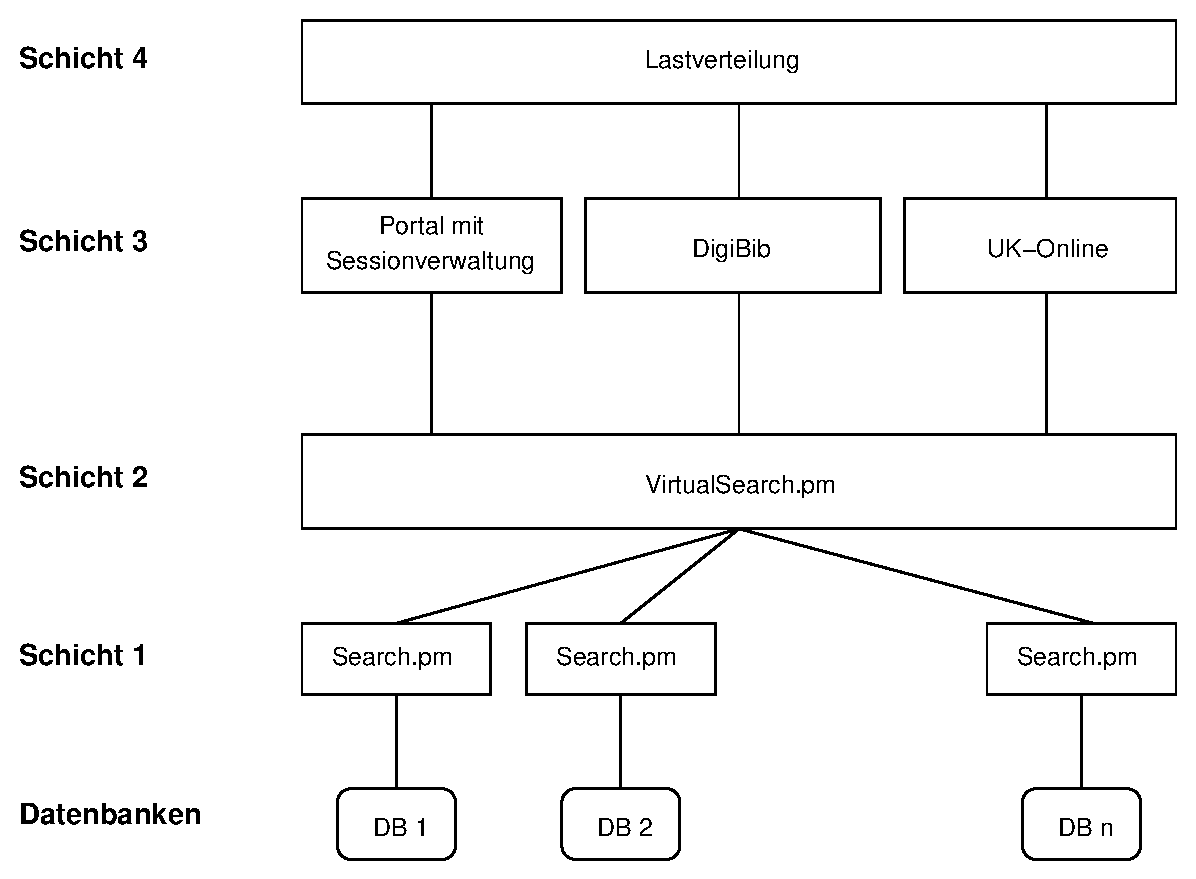
\includegraphics[width=12cm]{schicht04.eps}
    \end{minipage}
    \caption{Generelle Architektur der OpenBib-Portal-Suite}
  \label{bild:architektur}
  \vspace{3mm}
\end{shadowenv}
\end{figure}

\section{Die datenbankabh"angige Schicht 1 -- \texttt{OpenBib::Search}}

In der untersten, der datenbankabh"angigen Schicht greift das
Perl-Modul \texttt{OpenBib::Search} auf eine feste Datenbank zu.
Welche Datenbank dies ist, kann als Aufrufparamter dem Programm
mitgegeben werden. Dadurch ist es m"oglich, das gleiche Programm f"ur
Recherchen "uber ver\-schie\-de\-ne Daten\-banken zu nutzen. Das Modul
selbst -- wie auch alle anderen unter
\begin{verbatim}
openbib/portal/perl/modules
\end{verbatim}
angesiedelten Module -- ist als Erweiterung des Apache-Webservers via
\texttt{mod\_perl} realisiert.  Dadurch arbeitet es au"ser\-ordentlich
schnell.


\section{Die datenbank"ubergreifende Recherche-Schicht 2 -- \texttt{OpenBib::VirtualSearch}}

Die datenbank"ubergreifende Recherche geschieht in der "uber
\texttt{OpenBib::Search} liegenden Schicht 2 (vgl. Abb.
\ref{bild:architektur}) mit dem Perl-Modul
\texttt{OpenBib::VirtualSearch}. Aufgabe dieses Modules ist es, eine
Suchanfrage und eine Anzahl an Recherche-Datenbanken vom Benutzer
entgegen\-zuneh\-men und genau diese eine Suchanfrage sequentiell an
jede der "ubergebenen Datenbanken zu schicken. Zu diesem Zweck werden
entsprechende Utility-Routinen aus dem im
\texttt{OpenBib::Search}-Kontext angesiedelten Modul
\texttt{OpenBib::Search::Util} verwendet.

Die Ergebnisse der einzelnen Recherchen werden entgegengenommen und in
Listenform auf\-be\-rei\-tet. Die jeweiligen Titel selbst sind in dieser
Gesamttrefferliste via URL mit einer Suchanfrage f"ur genau diesen
Einzeltreffer mit \texttt{OpenBib::Search} verkn"upft. 
Bei der
Auswahl eines einzelnen Treffers wird dadurch direkt in die
zugeh"orige Datenbank via \texttt{OpenBib::Search} gesprungen. 

Alle 'normalen' Verkn"upfungs-Links (Normdaten, Hierarchien, etc.)
beziehen sich -- wir befinden uns nach der Auswahl eines Treffer wieder in
Schicht 1 -- auf genau diese eine Datenbank. "Uber das gro"se
stilisierte 'G' bei den Normdaten kann jedoch auch an dieser Stelle
wieder eine datenbank"ubergreifende Recherche nach genau dem
zugeh"origen Begriff gestartet werden. Der Benutzer hat somit bei
einem Einzeltreffer immer die M"oglichkeit selbst zu entscheiden, ob
er sich bzgl. der Normdaten weiter im zugeh"origen Katalog aufhalten
m"ochte, oder katalog"ubergreifend Recherchieren m"ochte.

Da in jedem Katalog die Verkn"upfungen bereits in der Datenbank
existieren, ist ein 'sich treiben lassen' in einem festen Katalog
au"ser\-ordentlich schnell, w"ahrend bei einer katalog"ubergreifenden
Suche ein kleiner Tribut zu zahlen ist, da nun effektiv wieder alle
Datenbanken mit einer 'neuen Suche' abgefragt werden.

Da \texttt{OpenBib::VirtualSearch} letztlich f"ur die
datenbank"ubergreifende Gewinnung der Recherche\-er\-geb\-nisse
zust"andig ist, werden nach erfolgreicher Recherche die Ergebnisse
aufgeteilt nach den einzelnen Katalogen in der Session-Datenbank
\texttt{session} 'gecached'. Durch das Caching der
Re\-cher\-che\-ergebnisse kann im Kontext von der Portal-Schicht 3
"ueber das dort angesiedelte Modul \texttt{OpenBib::ResultLists} auch
eine Trefferlistenfunktionalit"at geleistet werden, in der man "uber
die Ergebnisse der letzten Recherche hinaus auch noch direkt auf die
Ergebnisse jeder zuvor eingegebenen Suche in der aktuellen Session
zugreifen kann.

\section{Die Portal-Schicht 3 mit weiteren externen Zugriffmechanismen}

\subsection{Das Portal mit Session- und Benutzerverwaltung}

In der Portalschicht wird dem Benutzer sessionbasiert in einer aus
zwei Frames bestehenden Web-Seite eine Arbeits- und Recherche-Oberfl"ache
geliefert. 

Der Einsprung-URL in das Portal wird durch das Modul
\texttt{OpenBib::StartOpac} realisiert.

Das Modul \texttt{OpenBib::StartOpac} kann "uber verschiedene
Parameter gesteuert werden, die z.B. f"ur den direkten Sprung zu einem
einzelnen Treffer einer Datenbank oder der Anzeige einer
katalogeigenen Sicht des Portals Verwendung finden und gegebenenfalls
an nachgelagerte Module durchgereicht werden. Seine wesentliche
Aufgabe ist jedoch, eine eindeutige Session-ID zu generieren sowie ein
Frameset mit zwei Frames bereitzustellen.  Das obere Frame f"ur die
Navigation wird durch das Modul \texttt{OpenBib::HeaderFrame}
gef"ullt, das untere Frame standardm"a"sig zuerst durch das Modul
\texttt{OpenBib::SearchFrame}, das dem Navigations-Element 'Einfache
Recherche' bzw. 'Komplexe Recherche' entspricht.

Das Modul \texttt{OpenBib::HeaderFrame} ist f"ur die Navigation im Portal
inklusive Counter f"ur die Merkliste zust"andig.

In der Navigation werden folgende Funktionalit"aten angeboten:

\begin{description}
\item[Katalogauswahl] Die Auswahl der zu durchsuchenden Kataloge geschieht
  "uber eine entsprechende Aus\-wahl\-seite, die durch das Modul
  \texttt{OpenBib::DatabaseChoice} generiert wird.
\item[Recherche] Die Recherche-Maske wird "uber einen Aufruf von
  \texttt{OpenBib::SearchFrame} dargestellt.
\item[Trefferliste] Ein Zugriff auf Trefferlisten aus vorangegangenen
  Recherchen geschieht "uber das Modul \texttt{OpenBib::ResultLists},
  welches neben der verteilten Recherche auch f"ur ein Caching der
  Ergebnis-Daten zust"andig ist.
\item[Merkliste] Die Anzeige, Organisation sowie der Mailversand der
  Merkliste wird durch die Module
  \texttt{OpenBib::ManageCollection} und \texttt{OpenBib::MailCollection}
  "uber\-nom\-men. Bei Auswahl eines Treffers f"ur die Merkliste wird
  \texttt{OpenBib::HeaderFrame} aktualisiert, und zeigt die neue Zahl
  gemerkter Treffer an.
\item[RSS] "Uber das Modul \texttt{OpenBib::RSSFrame} wird eine zu
  diesem View zugeordnete Liste an RSS-Feeds f"ur die letzten 50
  Neuaufnahmen der entsprechenden Kataloge ausgegeben.
\item[Mein OpenBib] "Uber das Modul \texttt{OpenBib::Login}
  kann sich der Benutzer am Portal authentifizieren und so von
  weiteren personalisierten Funktionalit"aten profitieren. Dazu
  geh"oren neben generellen Benutzereinstellungen
  (\texttt{OpenBib::UserPrefs}) u.a. per\-sis\-ten\-te Merklisten sowie
  Datenbankprofile (\texttt{OpenBib::DatabaseProfile}).

  Das Modul gew"ahrt dabei den Zugang auf Grundlage seiner eigenen
  Datenbank, die "uber das Modul \texttt{OpenBib::SelfReg} via
  Selbstregistierung gef"ullt wird, bzw. auf Grundlage von lokalen
  Bibliothekssystemen -- hier wird konkret das Bibliothekssystem Sisis
  SunRise unterst"utzt --, die "uber eine selbst entwicklte
  WebServices-Schnittstelle OLWS (Open Library WebServices)
  angesprochen werden k"onnen. Falls ein Benutzer sein
  selbstregistriertes Passwort vergessen hat, so kann er es sich "uber
  das Modul \texttt{OpenBib::MailPassword} per Mail zusenden lassen.
\item[Hilfe] Die Hilfeseite wird direkt als URL
  \texttt{/suchhilfe.html} angesprochen.
\item[Sitzung beenden] Beim Ende der Sitzung wird zum Modul
  \texttt{OpenBib::Leave} gesprungen, welches die sessionrelevanten Daten
  entfernt sowie einen URL in die Schicht 4 zur Lastver\-teilungs\-instanz
  \texttt{OpenBib::LoadBalancer} mit Angabe eines eventuell aktiven Views
  (Institutssicht) f"ur einen er\-neu\-ten Einstieg in das Such-Portal
  bereitstellt.

\end{description}

\subsection{Externe Anbindung an die DigiBib}

Neben der Bereitstellung einer Recherche- und Arbeitsoberfl"ache f"ur
den Endbenutzer, besteht auch die M"oglichkeit "uber eine externe
Zugriffs-Schnittstelle automatisiert auf den Gesamtkatalog
zuzugreifen.

Eine solche M"oglichkeit besteht in der Einbindung in das Such-Portal
\textbf{Digitale Bibliothek NRW} (DigiBib) des
Hoch\-schul\-bibliotheks\-zentrum NRW (hbz). Das Suchinterface besteht aus
einem fest definierten Such-URL und einem fest definierten
HTML-basierten Antwortformat f"ur die Treffer. Grunds"atzlich wird auf
eine Rechercheanfrage, z.B. unter Angabe eines Suchbegriffes f"ur den
Titel, mit einer Kurztitelliste geantwortet. Es kann bestimmt werden,
welcher Teil der Kurztitelliste von den OpenBib-Daten\-banken
angefordert werden darf (Bl"atterfunktion mit frei w"ahlbarem Offset
und Schrittweite). Dar"uber hinaus wird neben der Kurztitelliste auch
die Anzeige eines Einzeltreffers mit weiter\-gehen\-den Kategorien
angeboten. In der Kurztitelliste sind alle Informationen vorhanden, um
den Einzeltreffer aufzurufen.

\subsection{Externe Anbindung an UK-Online}

Eine weitere Anbindung besteht in das Universit"atsportal UK-Online
von Herrn Prof. Lohnstein aus der Philosophischen Fakult"at der
Universit"at zu K"oln. Hier wird in UK-Online die M"oglichkeit
angeboten eigenen Bibliographie-Listen zu verwalten. Der Aufbau einer
solchen Bibliographie-Liste geschieht "uber die Recherche in OpenBib
und anschlie"sende Umwandlung und Ab\-spei\-cherung in ein
Bibliographie-Listen-Format.

Nach dem derzeitigen Stand sind beide externen Anbindung noch nicht in
einer lastverteilten Variante verf"ugbar. Diese ist jedoch kurz vor
der Fertigstellung.

\section{Die Lastverteilungs-Schicht 4}

Die Lastverteilungs-Schicht ist der erste Anlaufpunkt f"ur die
Benutzung von OpenBib. Diese Schicht wird f"ur das Portal durch das
Modul \texttt{OpenBib::LoadBalancer} und \texttt{OpenBib::ServerLoad} gebildet.
Entscheidungsgrundlage f"ur die Verteilung ist die Auslastung der
betroffenen Recher, deren generelle Ansprechbarkeit sowie die
generelle Funktionsf"ahigkeit des MySQL-Datenbanksystems.

Durch diese vorgeschaltete Verteilung der Recherche-Sitzungen auf
mehrere Rechner ergeben sich mehrere Vorteile:

\begin{enumerate}
\item Es wird eine Lastverteilung durchgef"uhrt. Wenn also ein Nutzer
  einen dieser URL's aufruft, so wird er auf den Rechner
  weitergeleitet, der am wenigsten belastet ist.  Dies ist prim"arer
  Zweck dieser Schicht.
\item Ist ein Rechner defekt -- im Sinne von 'nicht ansprechbar'
  bzw. 'DBMS-seitig nicht funktionsf"ahig' --, dann wird er bei der
  Verteilung/Weiterleitung nicht mehr ber"ucksichtigt und die Benutzer
  werden nur noch auf die verbliebenen Rechner verteilt. In diesem
  Fall ist bei der Weiterleitung mit einer kurzen Wartezeit von
  maximal 5 Sekunden (Timeout) zu rechnen.  Automatisch wird
  zus"atzlich an den Administrator eine Mail ge\-ne\-riert, die ihn
  auf den defekten Rechner hinweist. Ein Sonderfall ist natuerlich der
  'Verteilungs\-rech\-ner' selbst, bei dessen Ableben tempor"ar ein
  anderer Rechner unter seiner Identit"at einspringen mu"s. Letzteres
  kann selbstverst"andlich nicht automatisch geschehen und muss
  manuell konfiguriert werden. In diesem Sinn besteht mit dem
  Lastverteilungsrechner ein Singe-Point-Of-Failure, der nur "uber
  HA-Mechanismen ausger"aumt werden kann.
\item Werden Wartungsarbeiten auf einem der Rechner ausgef"uhrt, so
  kann man ihn selbst tempor"ar aus der Verteilung/Weiterleitung
  herausnehmen. Auf diese Weise "andert sich f"ur die Nutzer nichts,
  es werden dann die verbliebenen Rechner verwendet.
\end{enumerate}

\appendix

\chapter{Tabellen in \texttt{session.mysql}}

In diesem Anhang werden die einzelnen Tabellen in der
Session-Datenbank beschrieben.

Diese Tabellen verteilen sich auf rein session-basierte Aufgaben sowie
allgemeine Konfigurationseinstellungen des Portals.


\section{Tabellen zu session-basierten Aufgaben}

\begin{description}
\item[session] Dies ist die prim"are Tabelle in der die
  \texttt{sessionid} f"ur eine Nutzersitzung abgespeichert wird.
  Zus"atzlich werden folgende Informationen gespeichert:
  \begin{description}
  \item[createtime] Anfangszeit der Session.
  \item[lastresultset] Geordnete Liste der Katalog-ID's zur letzten
    Rechercheanfrage. Mit dieser Liste wird die katalog"ubergreifende
    Titelnavigation in der Einzeltrefferanzeige realisiert.
  \item[queryoptions] Allgemeine Suchoptionen. Durch die zentrale Speicherung der
    Suchoptionen brauchen diese nicht bei den internen URL-Verweisen
    verwendet werden.
  \end{description}
die Anfangszeit der Session \texttt{createtime}
  gespeichert. 
\item[treffer] Diese Tabelle realisiert sessionabh"angig die
  \textbf{Merkliste}. Es werden zu jeder Session der Datenbankname sowie die
  Identifikations-Nr des gemerkten Titels abgespeichert. Anhand dieser
  Informationen wird die Merkliste bei ihrem Aufruf sekundenaktuell
  mit dem etwaig vorhandenen Ausleihstatus der entsprechenden
  Titels"atze aufgebaut.
\item[sessionlog] Diese Tabelle soll im Betrieb mit relevanten
  Informationen gef"ullt werden, die dann statistisch ausgewertet
  werden k"onnen. Derzeit wird sie nicht verwendet.
\item[queries] In dieser Tabelle werden sessionabh"angig die
  Suchanfragen inkl. gefundener Treffer ab\-ge\-spei\-chert. Dadurch ist es
  m"oglich, sich "altere Suchanfragen wieder in die Recherchemaske
  eintragen zu lassen.
\item[dbchoice] In dieser Tabelle wird die vom Benutzer vorgenommene
  Datenbankauswahl session\-ab\-h"angig abgespeichert.
\item[searchresults] In dieser Tabelle wird session\-ab\-h"an\-gig zu jeder
  Suchanfrage (\texttt{queryid} der \texttt{queries}-Tabelle) pro
  Datenbank das Ergebnis gecached. Zus"atzlich wird jeweils auch noch
  die Anzahl der Treffer in der jeweiligen Datenbank
  ab\-ge\-spei\-chert. Durch diese Tabelle in Verbindung mit der Tabelle
  \texttt{queries} wird die \textbf{Trefferliste} realisiert.
\item[sessionview] "Uber diese Tabelle wird die Nutzung eines Views
  durch eine Session festgehalten. Diese Information wird ben"otigt,
  damit im oberen Frame (\texttt{OpenBib::HeaderFrame}) wie auch in der
  Recherchemaske (\texttt{OpenBib::SearchFrame}) die View-Informationen
  zus"atzlich angezeigt werden. Derzeit wird in \texttt{OpenBib::HeaderFrame}
  auf ein Bild mit dem Namen des Views
\begin{verbatim}
HTDOCS/images/openbib/views/<viewname>.png
\end{verbatim}

  verwiesen.
\item[sessionmask] In dieser Tabelle wird festgehalten, welche
  Recherchemaske -- Einfache Recherche oder Komplexe Recherche -- der
  Nutzer zuletzt aktiviert hat. Bei einer Aktivierung des allgemeinen
  Ober-Menueintrags 'Recherche' wird dann diese konkrete
  Recherchemaske ausgegeben.
\item[sessionprofile] \dots
\end{description}

\section{Tabellen zu allgemeinen Konfigurationseinstellungen des Portals}

\begin{description}
\item[dbinfo] In dieser Tabelle werden Informationen zu den einzelnen
  Katalogdatenbanken ab\-ge\-spei\-chert. Dazu geh"ort die Fakult"at
  (\texttt{faculty}, derzeit fest in den Modulen einprogrammiert),
  eine Beschreibung (\texttt{description}), das Katalogisierungssystem
  (\texttt{system} anhand K"urzel), der Datenbankname
  (\texttt{dbname}), das Bibliothekssigel (\texttt{sigel}) und
  schlie"slich die wesentliche Information, ob die Datenbank im Portal
  aktiv ist oder nicht (\texttt{active}). "Uber die letzte Einstellung
  lassen sich im laufenden Betrieb Datenbanken ein- und ausblenden.
\item[dboptions] Zu jeder Datenbank werden hier Informationen
  abgelegt, wo die zum Aufbau der Datenbank notwendigen Daten liegen
  und alle zum Heranschaffen der Daten ben"otigten Informationen wie
  Rechnername (\texttt{host}), Pfade, Dateinamen, Zugriffsprotokoll
  (\texttt{lokal}, \texttt{http}, \texttt{ftp}) und
  Authentifizierungsinformationen wie Benutzernamen oder Passworte.
  Derzeit sind diese Informationen schon im Wesentlichen vorhanden,
  sie werden durch die automatischen Konvertierungsskripte jedoch noch
  nicht verwendet.
\item[titcount] In dieser Tabelle wird die Anzahl der Titel pro
  Datenbank festgehalten. Diese Information wird "uber das Modul
  \texttt{OpenBib::SearchFrame} f"ur den Benutzer ausgegeben. Das Setzen
  dieser Werte geschieht "uber die automatischen
  Konvertierungsskripte.
\item[rssfeeds] In dieser Tabelle werden alle verfuegbaren Typen an RSS-Feeds
  zu den einzelnen Datenbank aus \texttt{dbinfo} definiert. Die
  RSS-Feeds lassen sich hier nach deren Konfiguration generell
  aktivieren sowie deaktivieren.
\item[rsscache] Um die Antwortzeiten bei der Generierung eines
  RSS-Feeds zu minimieren, wird ein RSS-Cache mit einer
  Aktivit"atsdauer von 12 Stunden verwendet.
\item[viewinfo] In dieser Tabelle werden zu einer Recherche-Sicht
  (view) neben dem den View de\-fi\-nier\-enden Viewnamen
  (\texttt{viewname}) auch eine Beschreibung \texttt{description}
  abgelegt. Die Informatione, ob der View aktiv ist oder nicht
  (\texttt{active}) wird derzeit nicht genutzt.
\item[viewdbs] In dieser Tabelle werden zu dem Viewnamen die Datenbanken
  festgelegt, die mit der konkreten Recherche-Sicht assoziiert
  sind. Hier k"onnen auch mehrere Datenbanken ein\-ge\-tra\-gen werden.
\item[viewrssfeeds] In dieser Tabellen werden zu einem View die
  RSS-Feeds konfiguriert, die in diesem View "uber den Menu-Punkt
  \texttt{RSS} angezeigt werden sollen

\end{description}



\chapter{Tabellen in \texttt{pool.mysql}}

Die Tabellen in \texttt{pool.mysql} werden nach Norm- bzw.
Stamm-Dateien geordnet dargestellt. Es sind dies \emph{Titel},
\emph{Verfasser}, \emph{K"orperschaften}, \emph{Notationen},
\emph{Schlagworte} sowie \emph{Exemplardaten}. Dar"uber hinaus gibt es eine zus"atzliche
Tabelle \texttt{search} in der in Form einer Volltextsuche
recherchiert werden kann. Verkn"upfungen zwischen den Norm-Dateien
werden "uber die Tabelle \texttt{conn} abgebildet.

\section{Titel-Normdaten}

\begin{description}
\item[tit] In dieser Tabelle befinden sich die f"ur die Anzeige
  bestimmten Titeldaten. Grunds"atzlich werden in dieser Tabelle
  folgende Informationen in einem Metadaten-unabh"angigen Format
  abgelegt.
  \begin{description}
  \item[id] Identifikationsnummer
  \item[category] Kategoriename -- sie basiert auf auf MAB2-Kategorienummer
  \item[indicator] Indikator -- transformiert von alphabetisch nach numerisch
  \item[content] Eigentlicher Kategorieinhalt
  \end{description}
\item[tit\_ft] Kategorien, die "uber einen Volltextindex recherchierbar
  gemacht werden.
  \begin{description}
  \item[id] Identifikationsnummer
  \item[category] Kategoriename -- sie basiert auf auf MAB2-Kategorienummer
  \item[content] Eigentlicher Kategorieinhalt, der suchbar gemacht wird.
  \end{description}
\item[tit\_string] Kategorien, die "uber eine Wortanfangssuche
  recherchierbar gemacht werden.
  \begin{description}
  \item[id] Identifikationsnummer
  \item[category] Kategoriename -- sie basiert auf auf MAB2-Kategorienummer
  \item[content] Eigentlicher Kategorieinhalt, der suchbar gemacht wird.
  \end{description}
\end{description}

\section{Verfasser-Normdaten}

\begin{description}
\item[aut] In dieser Tabelle befinden sich die f"ur die Anzeige
  bestimmten Verfasserinformationen f"ur die Kategorien
  \textbf{Verfasser} und \textbf{Person}. Grunds"atzlich werden in
  dieser Tabelle folgende Informationen in einem
  Metadaten-unabh"angigen Format abgelegt.
  \begin{description}
  \item[id] Identifikationsnummer
  \item[category] Kategoriename -- eigentlich eine interne Kategorienummer
  \item[indicator] Indikator -- transformiert von alphabetisch nach numerisch
  \item[content] Eigentlicher Kategorieinhalt
  \end{description}
\item[aut\_ft] Kategorien, die "uber einen Volltextindex recherchierbar
  gemacht werden.
  \begin{description}
  \item[id] Identifikationsnummer
  \item[category] Kategoriename -- eigentlich eine interne Kategorienummer
  \item[content] Eigentlicher Kategorieinhalt, der suchbar gemacht wird.
  \end{description}
\item[aut\_string] Kategorien, die "uber eine Wortanfangssuche
  recherchierbar gemacht werden.
  \begin{description}
  \item[id] Identifikationsnummer
  \item[category] Kategoriename -- eigentlich eine interne Kategorienummer
  \item[content] Eigentlicher Kategorieinhalt, der suchbar gemacht wird.
  \end{description}
\end{description}

\section{K"orperschafts-Normdaten}

\begin{description}
\item[kor] In dieser Tabelle befinden sich die f"ur die Anzeige
  bestimmten K"orperschaftsinformationen f"ur die Kategorien
  \textbf{K"orperschaft} und \textbf{Urheber}. Grunds"atzlich werden in
  dieser Tabelle folgende Informationen in einem
  Metadaten-unabh"angigen Format abgelegt.
  \begin{description}
  \item[id] Identifikationsnummer
  \item[category] Kategoriename -- eigentlich eine interne Kategorienummer
  \item[indicator] Indikator -- transformiert von alphabetisch nach numerisch
  \item[content] Eigentlicher Kategorieinhalt
  \end{description}
\item[kor\_ft] Kategorien, die "uber einen Volltextindex recherchierbar
  gemacht werden.
  \begin{description}
  \item[id] Identifikationsnummer
  \item[category] Kategoriename -- eigentlich eine interne Kategorienummer
  \item[content] Eigentlicher Kategorieinhalt, der suchbar gemacht wird.
  \end{description}
\item[kor\_string] Kategorien, die "uber eine Wortanfangssuche
  recherchierbar gemacht werden.
  \begin{description}
  \item[id] Identifikationsnummer
  \item[category] Kategoriename -- eigentlich eine interne Kategorienummer
  \item[content] Eigentlicher Kategorieinhalt, der suchbar gemacht wird.
  \end{description}
\end{description}

\section{Schlagwort-Normdaten}

\begin{description}
\item[swt] In dieser Tabelle befinden sich die f"ur die Anzeige
  bestimmten K"orperschaftsinformationen f"ur die Kategorie
  \textbf{Schlagwort}. Grunds"atzlich werden in dieser Tabelle
  folgende Informationen in einem Metadaten-unabh"angigen Format
  abgelegt.
  \begin{description}
  \item[id] Identifikationsnummer
  \item[category] Kategoriename -- eigentlich eine interne Kategorienummer
  \item[indicator] Indikator -- transformiert von alphabetisch nach numerisch
  \item[content] Eigentlicher Kategorieinhalt
  \end{description}
\item[swt\_ft] Kategorien, die "uber einen Volltextindex recherchierbar
  gemacht werden.
  \begin{description}
  \item[id] Identifikationsnummer
  \item[category] Kategoriename -- eigentlich eine interne Kategorienummer
  \item[content] Eigentlicher Kategorieinhalt, der suchbar gemacht wird.
  \end{description}
\item[swt\_string] Kategorien, die "uber eine Wortanfangssuche
  recherchierbar gemacht werden.
  \begin{description}
  \item[id] Identifikationsnummer
  \item[category] Kategoriename -- eigentlich eine interne Kategorienummer
  \item[content] Eigentlicher Kategorieinhalt, der suchbar gemacht wird.
  \end{description}
\end{description}

\section{Notations-Normdaten}

\begin{description}
\item[notation] In dieser Tabelle befinden sich die f"ur die Anzeige
  bestimmten Notationsinformationen f"ur die Kategorie
  \textbf{Notation}. Grunds"atzlich werden in dieser Tabelle
  folgende Informationen in einem Metadaten-unabh"angigen Format
  abgelegt.
  \begin{description}
  \item[id] Identifikationsnummer
  \item[category] Kategoriename -- eigentlich eine interne Kategorienummer
  \item[indicator] Indikator -- transformiert von alphabetisch nach numerisch
  \item[content] Eigentlicher Kategorieinhalt
  \end{description}
\item[notation\_ft] Kategorien, die "uber einen Volltextindex recherchierbar
  gemacht werden.
  \begin{description}
  \item[id] Identifikationsnummer
  \item[category] Kategoriename -- eigentlich eine interne Kategorienummer
  \item[content] Eigentlicher Kategorieinhalt, der suchbar gemacht wird.
  \end{description}
\item[notation\_string] Kategorien, die "uber eine Wortanfangssuche
  recherchierbar gemacht werden.
  \begin{description}
  \item[id] Identifikationsnummer
  \item[category] Kategoriename -- eigentlich eine interne Kategorienummer
  \item[content] Eigentlicher Kategorieinhalt, der suchbar gemacht wird.
  \end{description}
\end{description}

\section{Exemplar-Daten}

\begin{description}
\item[mex] In dieser Tabelle befinden sich die f"ur die Anzeige
  bestimmten Exemplarinformationen aus dem Titeldatenbereich.
  Grunds"atzlich werden in dieser Tabelle folgende Informationen in
  einem Metadaten-unabh"angigen Format abgelegt.
  \begin{description}
  \item[id] Identifikationsnummer
  \item[category] Kategoriename -- eigentlich eine interne Kategorienummer
  \item[indicator] Indikator -- transformiert von alphabetisch nach numerisch
  \item[content] Eigentlicher Kategorieinhalt
  \end{description}
\item[mex\_ft] Kategorien, die "uber einen Volltextindex recherchierbar
  gemacht werden.
  \begin{description}
  \item[id] Identifikationsnummer
  \item[category] Kategoriename -- eigentlich eine interne Kategorienummer
  \item[content] Eigentlicher Kategorieinhalt, der suchbar gemacht wird.
  \end{description}
\item[mex\_string] Kategorien, die "uber eine Wortanfangssuche
  recherchierbar gemacht werden.
  \begin{description}
  \item[id] Identifikationsnummer
  \item[category] Kategoriename -- eigentlich eine interne Kategorienummer
  \item[content] Eigentlicher Kategorieinhalt, der suchbar gemacht wird.
  \end{description}
\end{description}

\section{Verkn"upfungen zwischen den Normdaten}

\begin{description}
\item[conn] In dieser Tabelle befinden sich
  Verkn"upfungsinformationen f"ur die Normdaten. 
  Grunds"atzlich werden in dieser Tabelle folgende Informationen in
  einem Metadaten-unabh"angigen Format abgelegt.
  \begin{description}
  \item[category] Kategorie(nummer), der die Verkn"upfung zugeordnet
    ist (z.B. Verfasser vs. Person)
  \item[sourceid] Id des zu verkn"upfenden Satzes
  \item[sourcetype] Normdatei des zu verkn"upfenden Satzes
  \item[targetid] Id des verkn"upften Satzes
  \item[targettype] Normdatei des verkn"upften Satzes
  \item[supplement] Zusatzinformation, die der Verkn"upfung zugeordnet
    ist (z.B. [Hrsg.])
  \end{description}
\end{description}


\section{Recherche-Tabelle \texttt{search}}

S"amtliche vom Benutzer eingegebenen Suchbegriffe werden in der Tabelle
\texttt{search} recherchiert. Als Ergebnis der Suche werden
Identifikationsnummern (IDN's, Katkeys) der gefundenen Titel-S"atze
zur"uckgeliefert. Mit diesen IDN's wird dann in die Norm- bzw.
Stammdateien gesprungen, um alle Informationen zu diesen Titel-S"atzen
zu gewinnen. Diese Funktionalit"at wird allein von dem Modul
\texttt{OpenBib::Search} geleistet.

\chapter{Module geordnet nach Funktion bzw. Schicht}


\section{Schicht"ubergreifend}


\begin{itemize}
\item \texttt{OpenBib::Config}
\end{itemize}

\section{Schicht 1 - Zugriff auf Katalogdatenbank}

\begin{itemize}
\item \texttt{OpenBib::Search}
\end{itemize}

\section{Schicht 2 - Zugriff auf versch. Datenbanken der Schicht 1}

\begin{itemize}
\item \texttt{OpenBib::VirtualSearch}
\end{itemize}

\section{Schicht 3 - Rechercheportal}

\begin{itemize}
\item \texttt{OpenBib::DatabaseChoice}
\item \texttt{OpenBib::DatabaseProfile}
\item \texttt{OpenBib::HeaderFrame}
\item \texttt{OpenBib::Leave}
\item \texttt{OpenBib::Login}
\item \texttt{OpenBib::MailCollection}
\item \texttt{OpenBib::MailPassword}
\item \texttt{OpenBib::ManageCollection}
\item \texttt{OpenBib::SearchFrame}
\item \texttt{OpenBib::SelfReg}
\item \texttt{OpenBib::StartOpac}
\item \texttt{OpenBib::UserPrefs}
\end{itemize}

\section{Schicht 4 - Lastverteilung}

\begin{itemize}
\item \texttt{OpenBib::LoadBalancer}
\item \texttt{OpenBib::ServerLoad}
\end{itemize}


\begin{thebibliography}{ChBr82}
\originalTeX

\bibitem[FliHof06]{FlimmHoffJB:06} O.~Flimm, Chr. Hoffrath: \emph{Der
    Weg des KUG zum umfassenden Recherche-Portal}; erscheint in:
  Kooperative Informationsverarbeitung an der Universität zu Köln -
  Bericht für das Jahr 2005 (2006).
\bibitem[BoeFli:06]{BoeFli:EinbandDB} R.~Boeff, O.~Flimm: \emph{Von
    der traditionellen zur digitalen Sammlung historischer und
    künstlerischer Bucheinbände der USB Köln mit einem Einblick in die
    technische Konzeption der Datenbank}. -- in: Bibliothek. Forschung
  und Praxis. Jahrgang 30 (2006) Nr. 1, S.63
\end{thebibliography}
\germanTeX

\end{document}